\documentclass[a4paper,10pt]{article}
\usepackage[utf8]{inputenc}
\usepackage[english,russian]{babel}
\usepackage{fancyhdr}
\usepackage{caption}
\usepackage{hyperref}

\usepackage{listings,longtable,amsmath,amsfonts,graphicx,tikz,tabularx,amssymb}
\usetikzlibrary{automata}
\usepackage{algpseudocode}
\usepackage{pgfplots}

\captionsetup{labelsep=period}
\pagestyle{fancy}

\lstset{
    basicstyle=\footnotesize,
    breakatwhitespace=false,
    breaklines=true,
    extendedchars=true,
    keepspaces=true,
    keywordstyle=\bfseries,
    numbers=left,
    numbersep=3pt,
    numberstyle=\tiny,
    showspaces=false,
    showstringspaces=false,
    showtabs=false,
    stepnumber=1,
    stringstyle=\emph,
    tabsize=2
}


\tikzset{
    min/.style = {circle, draw=gray,fill=gray, text=white, thick}
}

\usepackage[left=1.5cm,right=1.5cm,top=2cm,bottom=1.5cm,bindingoffset=0cm]{geometry}

\captionsetup{labelsep=period}
\pagestyle{fancy}

\renewcommand{\headrulewidth}{0pt}
\fancyfoot[L] {\thepage\bf}
\fancyfoot[C] {}

\graphicspath{ {img/} }

\begin{document}
    \begin{titlepage}
        \begin{center}
            \large
            САНКТ-ПЕТЕРБУРГСКИЙ НАЦИОНАЛЬНЫЙ ИССЛЕДОВАТЕЛЬСКИЙ УНИВЕРСИТЕТ ИНФОРМАЦИОННЫХ ТЕХНОЛОГИЙ, МЕХАНИКИ И ОПТИКИ \\
            \vspace{3cm}

            Кафедра вычислительной техники
            \vspace{4cm}

            \textsc{ \textbf{Отчёт по лабораторной работе  № 3} \\
            по дисциплине <<Тестирование программного обеспечения>>\\}

            \bigskip
        \end{center}
        \vspace{3cm}

        \hfill\begin{flushright}
             Студенты: \\ Куклина М. \\ Кириллова А. \\ гр. P3301
             \vfill
             Преподаватель: \\ Клименков C.В. 
        \end{flushright}
        \vfill
        \vfill
        \vfill
        \vfill
        \vfill
        \begin{center}
            Санкт-Петербург \\ 2017 г.
        \end{center}
    \end{titlepage}
\newpage

\section*{Задание}

    В ходе нагрузочного тестирования необходимо протестировать 3 конфигурации аппаратного обеспечения и выбрать среди них наиболее дешёвую, удовлетворяющую требованиям по максимальному времени отклика приложения при заданной нагрузке (в соответствии с вариантом).

    В ходе стресс-тестирования необходимо определить, при какой нагрузке выбранная на предыдущем шаге конфигурация перестаёт удовлетворять требованиями по максимальному времени отклика. Для этого необходимо построить график зависимости времени отклика приложения от нагрузки.
	
	Параметры:
	\begin{itemize}
        \item URL первой конфигурации (\$ 3600) --  \url{http://aqua:8080?token=440693507&user=1511647816&conf=1};
        \item URL второй конфигурации (\$ 7000) --   \url{http://aqua:8080?token=440693507&user=1511647816&conf=2};
        \item URL третьей конфигурации (\$ 11900) -- \url{http://aqua:8080?token=440693507&user=1511647816&conf=3};
        \item Максимальное количество параллельных пользователей - 11;
        \item Средняя нагрузка, формируемая одним пользователем - 20 запр. в мин.;
        \item Максимально допустимое время обработки запроса - 910 мс.
	\end{itemize}

\section*{Нагрузочное тестирование}
	\subsection*{Конфигурация JMeter}
		\begin{itemize}
			\item ThreadGroup:
				\begin{itemize}
                    \item Количество параллельных пользователей: users = 11;
                    \item Промежуток времени, через который запускается очередной пользователь: rump-up period = 0;
                    \item Количество выполнения сценария: loop count = 70.
				\end{itemize}
			\item Duration Assertion: duration = 910;
			\item Response Assertion: code != [503, 403];
			\item Constant Throughput Time: taget throughput = 20.
		\end{itemize}

	\subsection*{Нагрузочное тестирование конфигурации оборудования}
		\begin{figure}[h!]
			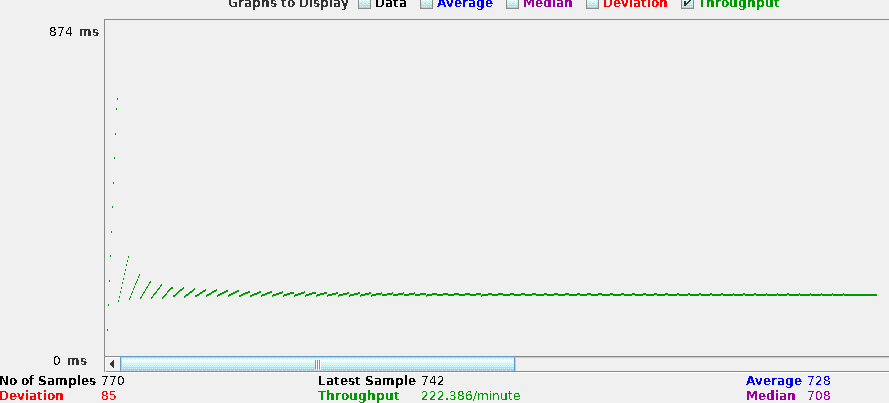
\includegraphics[scale=0.5]{./img/loadtest_conf1.png}
			\caption{Результат нагрузочного тестирования конфигурации 1}
		\end{figure}

		\begin{figure}[h!]
			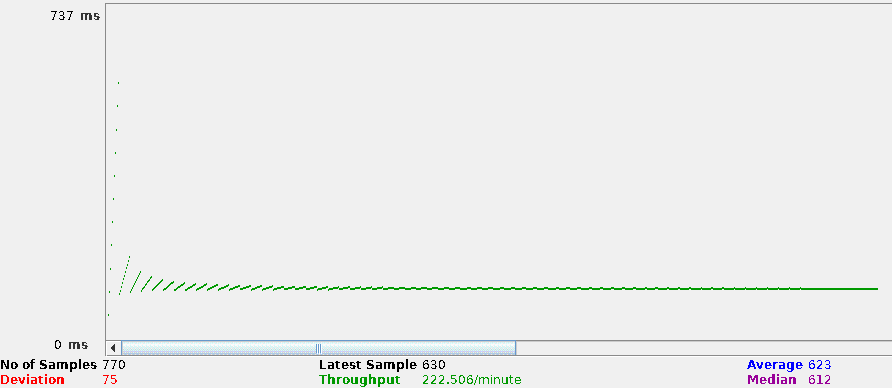
\includegraphics[scale=0.5]{./img/loadtest_conf2.png}
			\caption{Результат нагрузочного тестирования конфигурации 2}
		\end{figure}

		\begin{figure}[h!]
			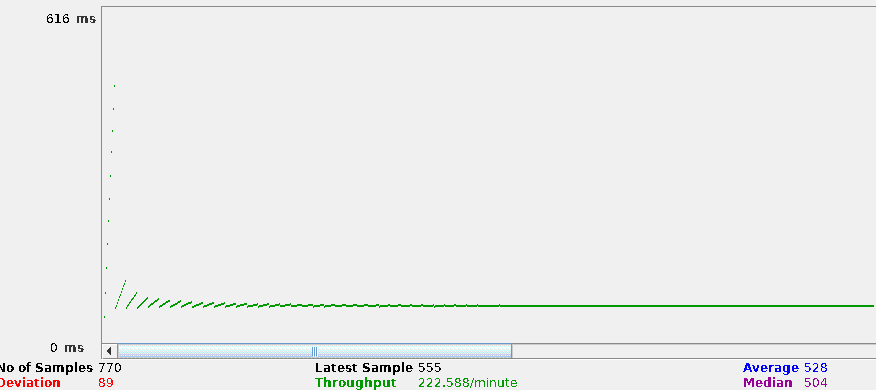
\includegraphics[scale=0.5]{./img/loadtest_conf3.png}
			\caption{Результат нагрузочного тестирования конфигурации 3}
		\end{figure}

\newpage

	\subsection*{Результаты}
	
	Ни одна из представленных конфигураций не содержит некорректные параметры, а также не превышает максимально
	допустимое время обработки в 910 мс. Из всех представленных конфигураций мы вбрали вторую в силу её
    приемлемого времени обработки и цены в сравнении с остальными вариантами.

\newpage

\section*{Стресс-тестирование выбранной конфигурации}

	\subsection*{Конфигурация JMeter}
		Аналогична конфигурации в первой части работы. Для создания графика использовался Response Time Graph listener.

	\subsection*{Стресс-тестирование выбранной конфигурации оборудования}
		\begin{figure}[h!]
			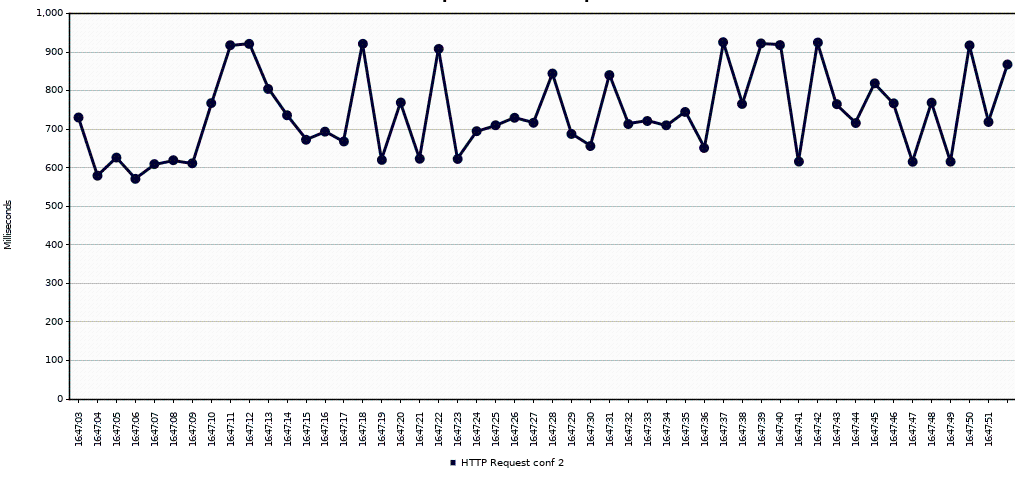
\includegraphics[scale=0.5]{./img/stresstest_conf2.png}
			\caption{Результат стресс-тестирования конфигурации 2}
		\end{figure}

	\subsection*{Результаты}

		При нагрузке 100 запросов в мин. обработка запроса начинает превышать максимальное время в 910 мс.

\section*{Вывод}

	В ходе выполнения лабораторной работы были преведены нагрузночное и стресс- тестирование заданных конфигураций
	оборудования. Ни одна конфигурация не содержала некорректные параметры, поэтому выбор наилучшего варианта
	был сделан на основе цены конфигурации и метрик, выявленных в результате тестирование. Таким вариантов оказалась
	вторая конфигурация, где соотношение цена/качество была наиболее оптимальной относительно других вариантов. 
	При стресс-тестировании варианта оказалось, что данная конфигурация выдерживает максимально до 100 запросов в минуту
	от одного пользователя.

\end{document}
